\LARGE
\begin{center}
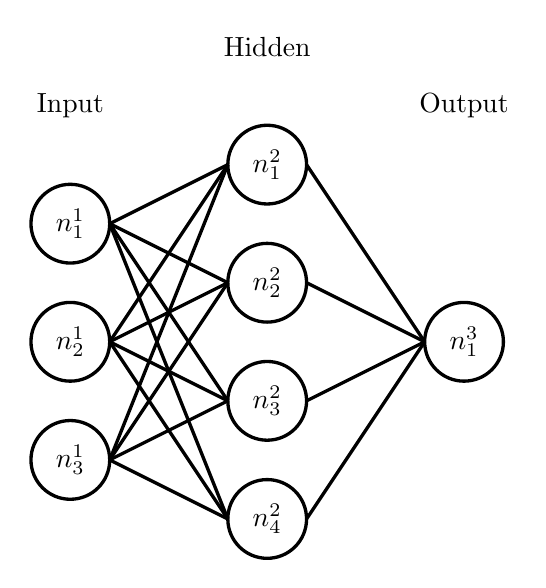
\begin{tikzpicture}

        \foreach \x in {1, 2, 3}
        {
                \draw[very thick] (0, -1.5*\x) circle (0.5);
                \node at (0, -1.5*\x) {$n_{\x}^1$};
                \foreach \y in {1, 2, 3, 4}
                {
                        \draw[very thick] (0.5, -1.5*\x) -- (2, -1.5*\y+0.75);
                }
        }

        \foreach \y in {1, 2, 3, 4}
        {
                \draw[very thick] (2.5, -1.5*\y+0.75) circle (0.5);
                \node at (2.5, -1.5*\y+0.75){$n_{\y}^2$};
                \draw[very thick] (3, -1.5*\y+0.75) -- (4.5, -3);
        }
        \draw[very thick] (5, -3) circle (0.5);
        \node at (5, -3){$n_1^3$};
        
        \node at (0, 0){Input};
        \node at (2.5, 0.75){Hidden};
        \node at (5, 0){Output};

\end{tikzpicture}
\end{center}
\normalsize
